\subsection{External interface Requirements}
The \emph{DREAM} frontend is a web application that can be accessed from web browsers, both from mobile and
desktop devices. The following section will give a comprehensive description in terms of hardware, software
and communication interfaces.

\bigskip
\subsubsection{Common users interfaces}
\textbf{Login and Registration}\\
When first opening the application, all the users are presented with the login page. If not already registered,
it is provided a registration button. In this section they are asked to provide: first name, second name,
a \emph{username}, an \emph{e-mail address} and a \emph{password}. The interface also shows a small button to switch
to the login page, in case the user has already signed in on another device or the session has expired.

\bigskip
\begin{figure}[H]
    \centering
    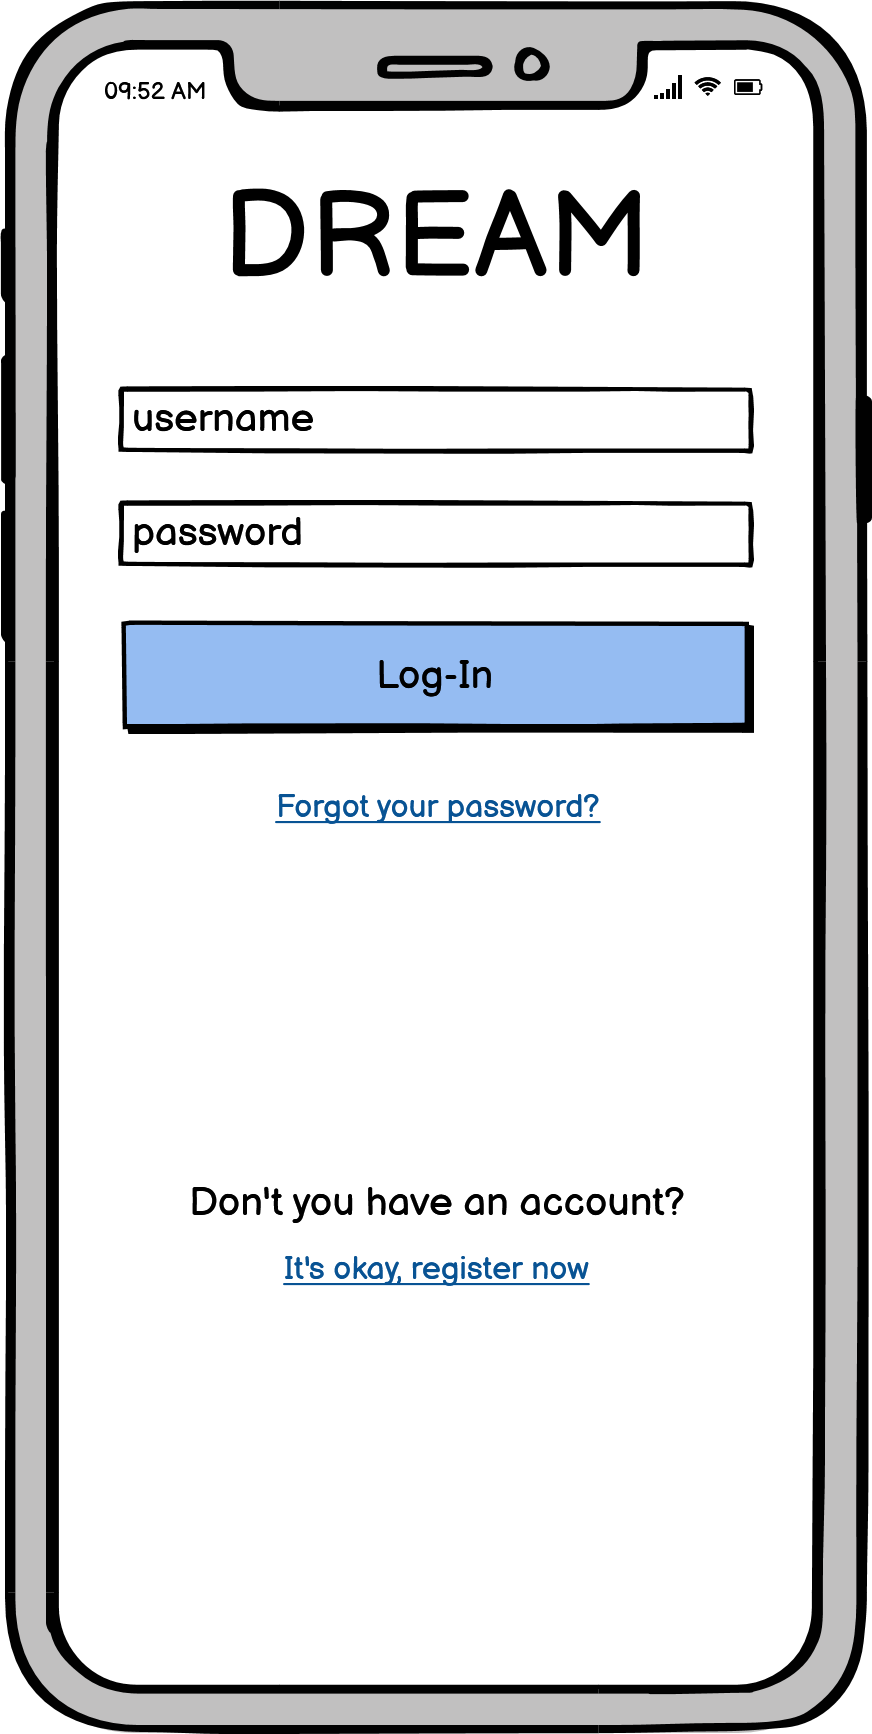
\includegraphics[scale=0.40]{Images/log-in.png}
    \caption{Log-in interface}
\end{figure}

\newpage
\begin{figure}[H]
    \centering
    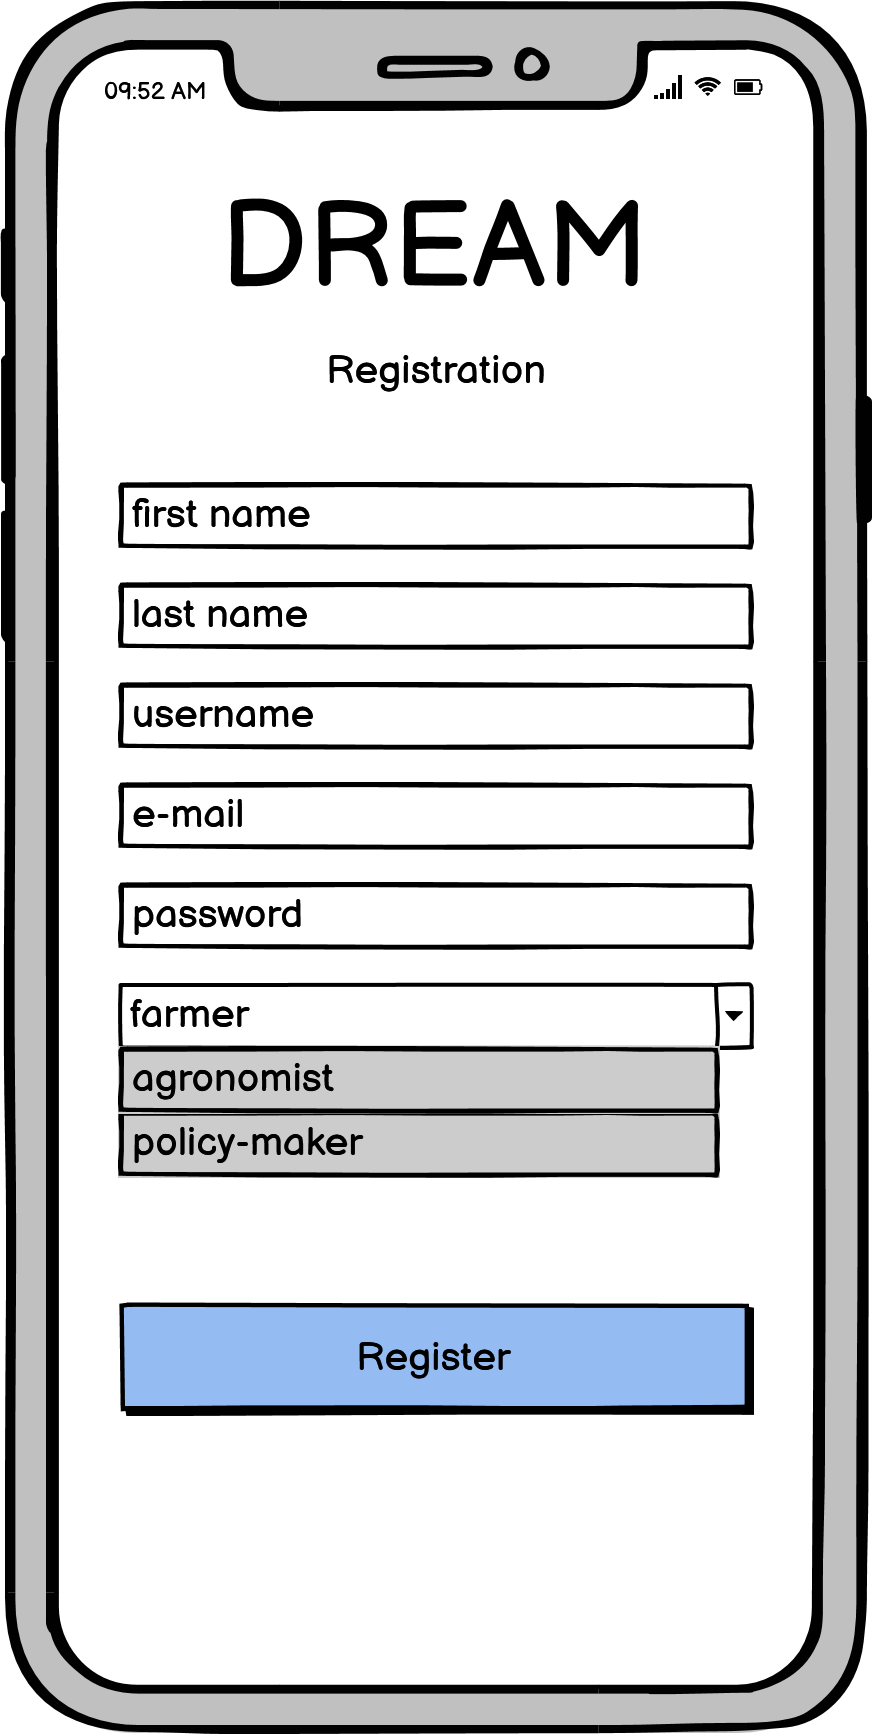
\includegraphics[scale=0.40]{Images/registration.png}
    \caption{Registration interface}
\end{figure}

\textbf{Farmer's home page} \\
Provides different options. The user can insert data concerning production,
checks weather forecasts, privately request help, and reach the forum.
\begin{figure}[H]
    \centering
    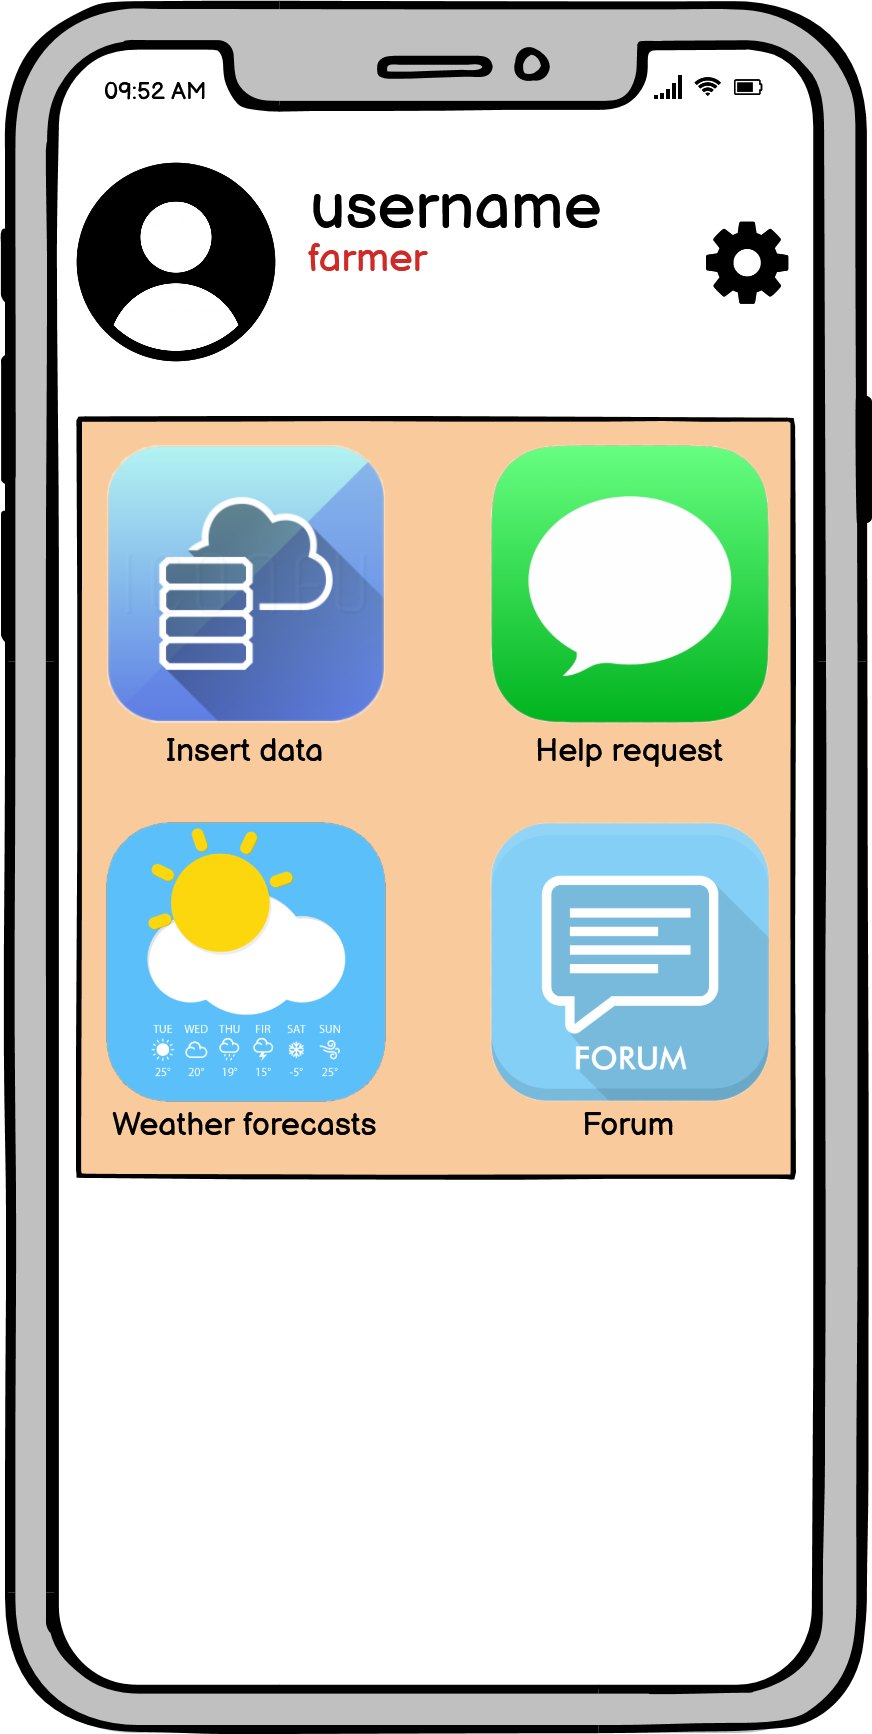
\includegraphics[scale=0.45]{Images/farmerHomePage.png}
    \caption{Farmer's home page}
\end{figure}

\textbf{Agronomist's home page} \\
Provides the possibility of selecting the area of responsibility, answering private help requests,
checking the weather, accessing the forum, managing the daily plan, and checking the dashboard
\begin{figure}[H]
    \centering
    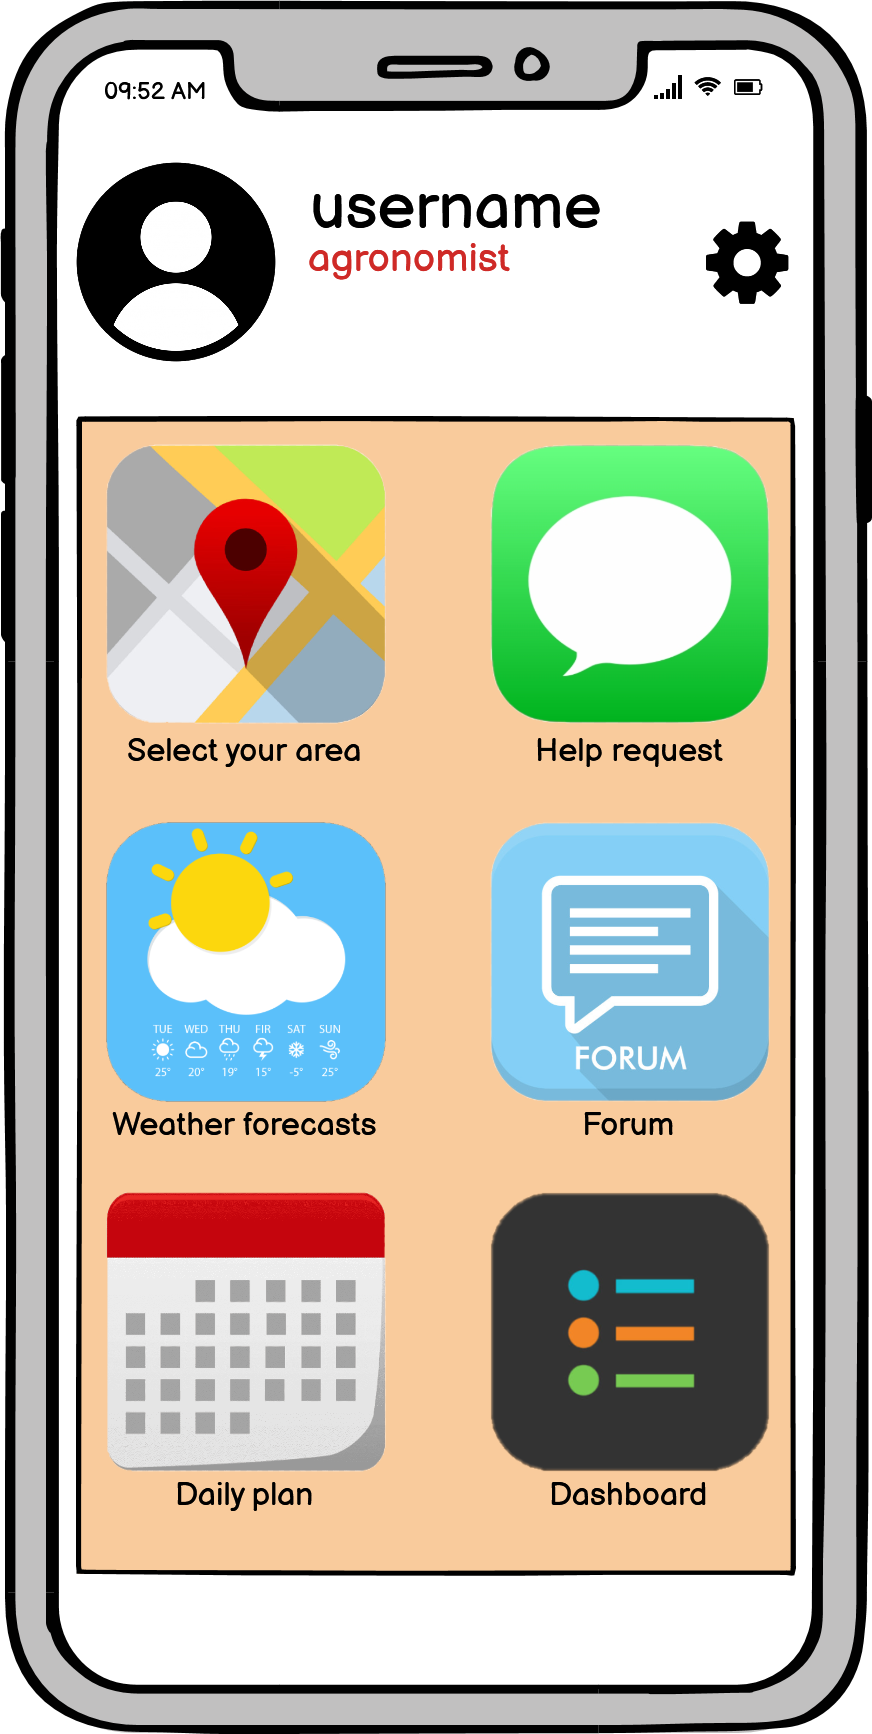
\includegraphics[scale=0.40]{Images/agronomistHomePage.png}
    \caption{Agronomist's home page}
\end{figure}

\textbf{Policymaker's home page} \\
Provides a table containing values for all farmers in the system. Every field of this table can be ordered.
\newline There are also graphs that sum up data about production.
\begin{figure}[H]
    \centering
    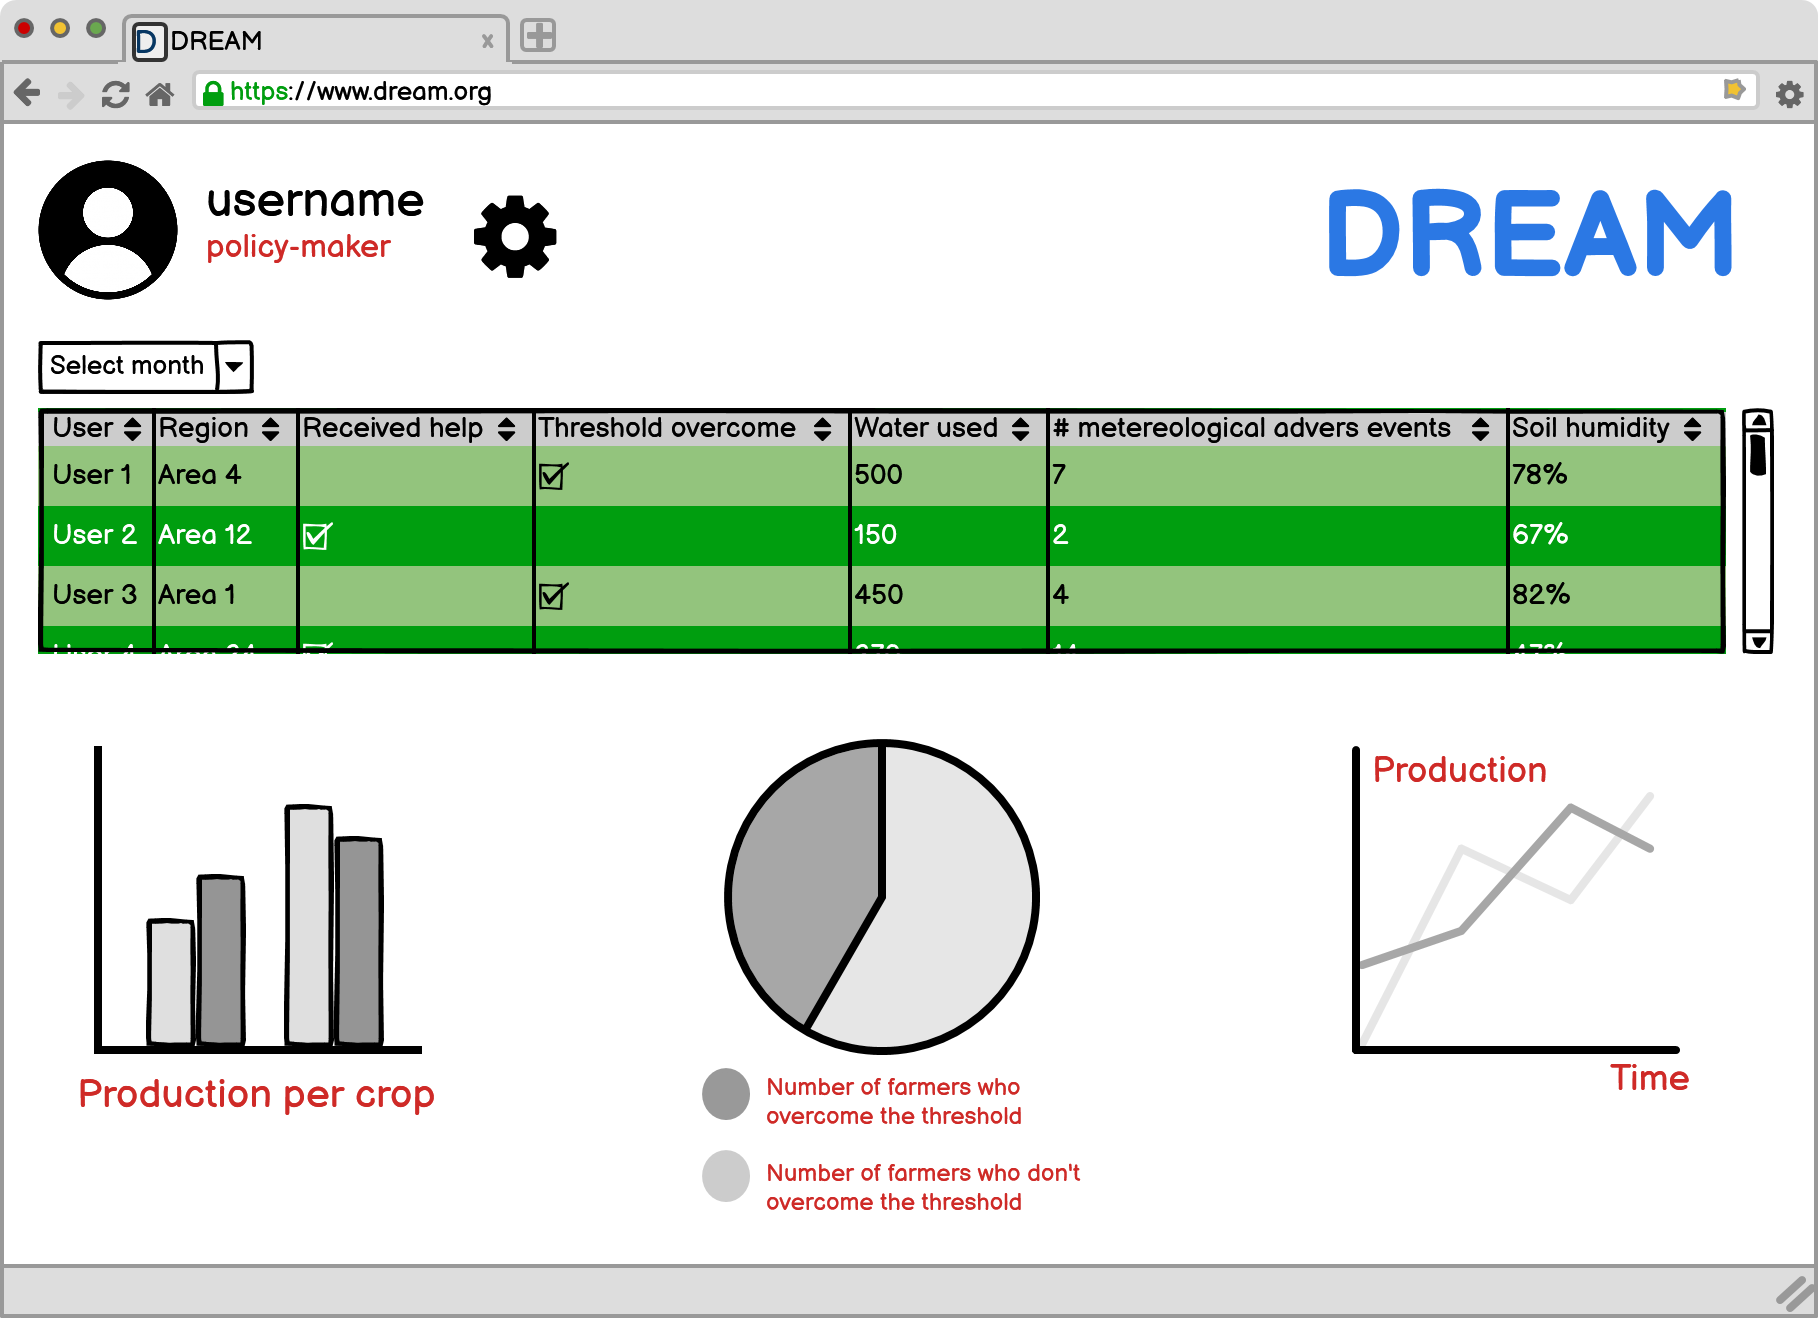
\includegraphics[scale=0.40]{Images/policymakerHomePage.png}
    \caption{Policymaker's home page}
\end{figure}

\newpage
\textbf{Forum - home page} \\
The forum section is accessible to both the farmers and the agronomists. Agronomists have the possibility
of taking a look at the requests and answer to them. Farmers, as agronomists, can answer to the forum threads
but can also create a new discussion.
\begin{figure}[H]
    \centering
    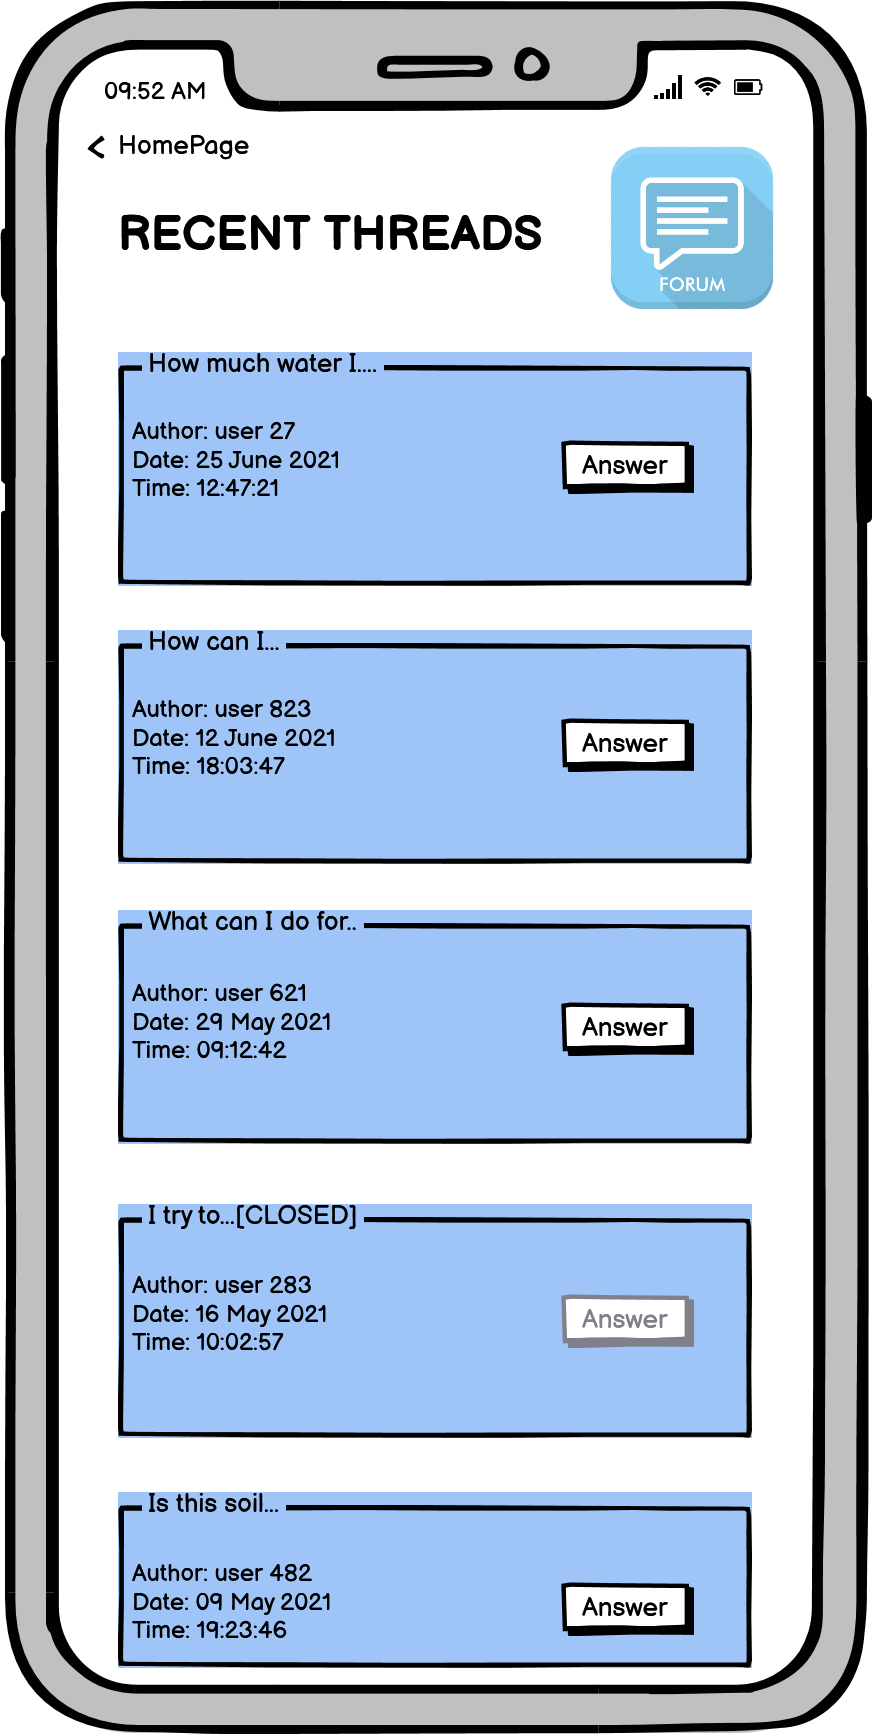
\includegraphics[scale=0.40]{Images/agronomistForum.png}
    \caption{Agronomist's forum home page}
\end{figure}
\bigskip
\begin{figure}[H]
    \centering
    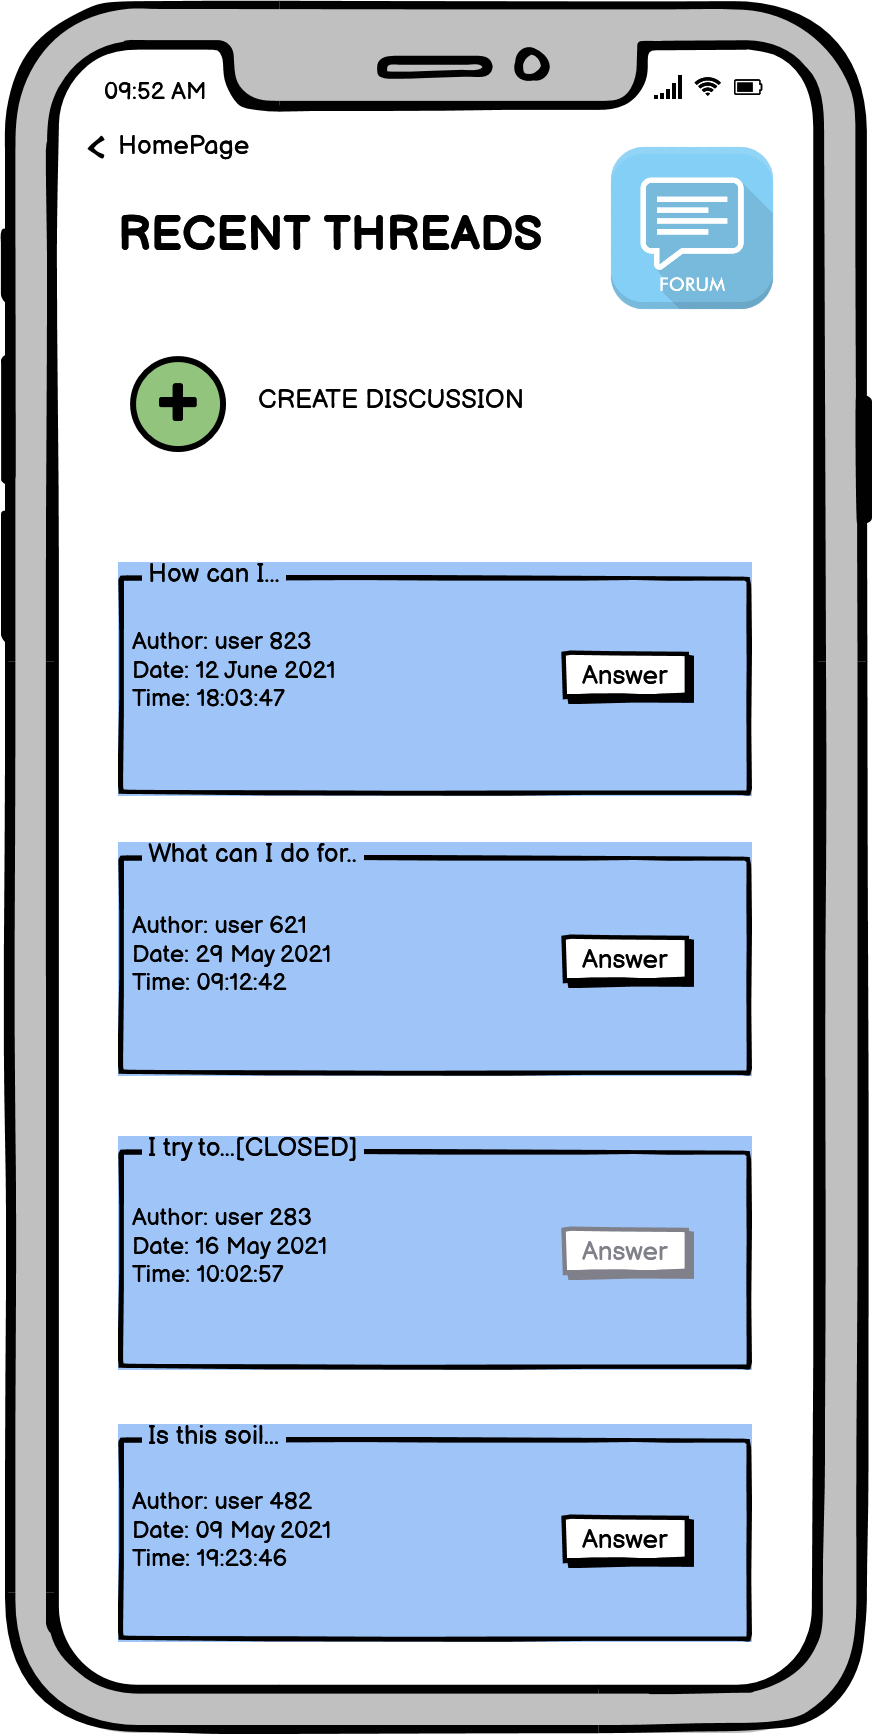
\includegraphics[scale=0.40]{Images/farmerForum.png}
    \caption{Farmer's forum home page}
\end{figure}

\newpage
\textbf{Daily plan - home page} \\
The daily plan home page presents a calendar in which appointments day are marked in red.
By clicking on a date is possible to manage it, by adding or removing an appointment.
\begin{figure}[H]
    \centering
    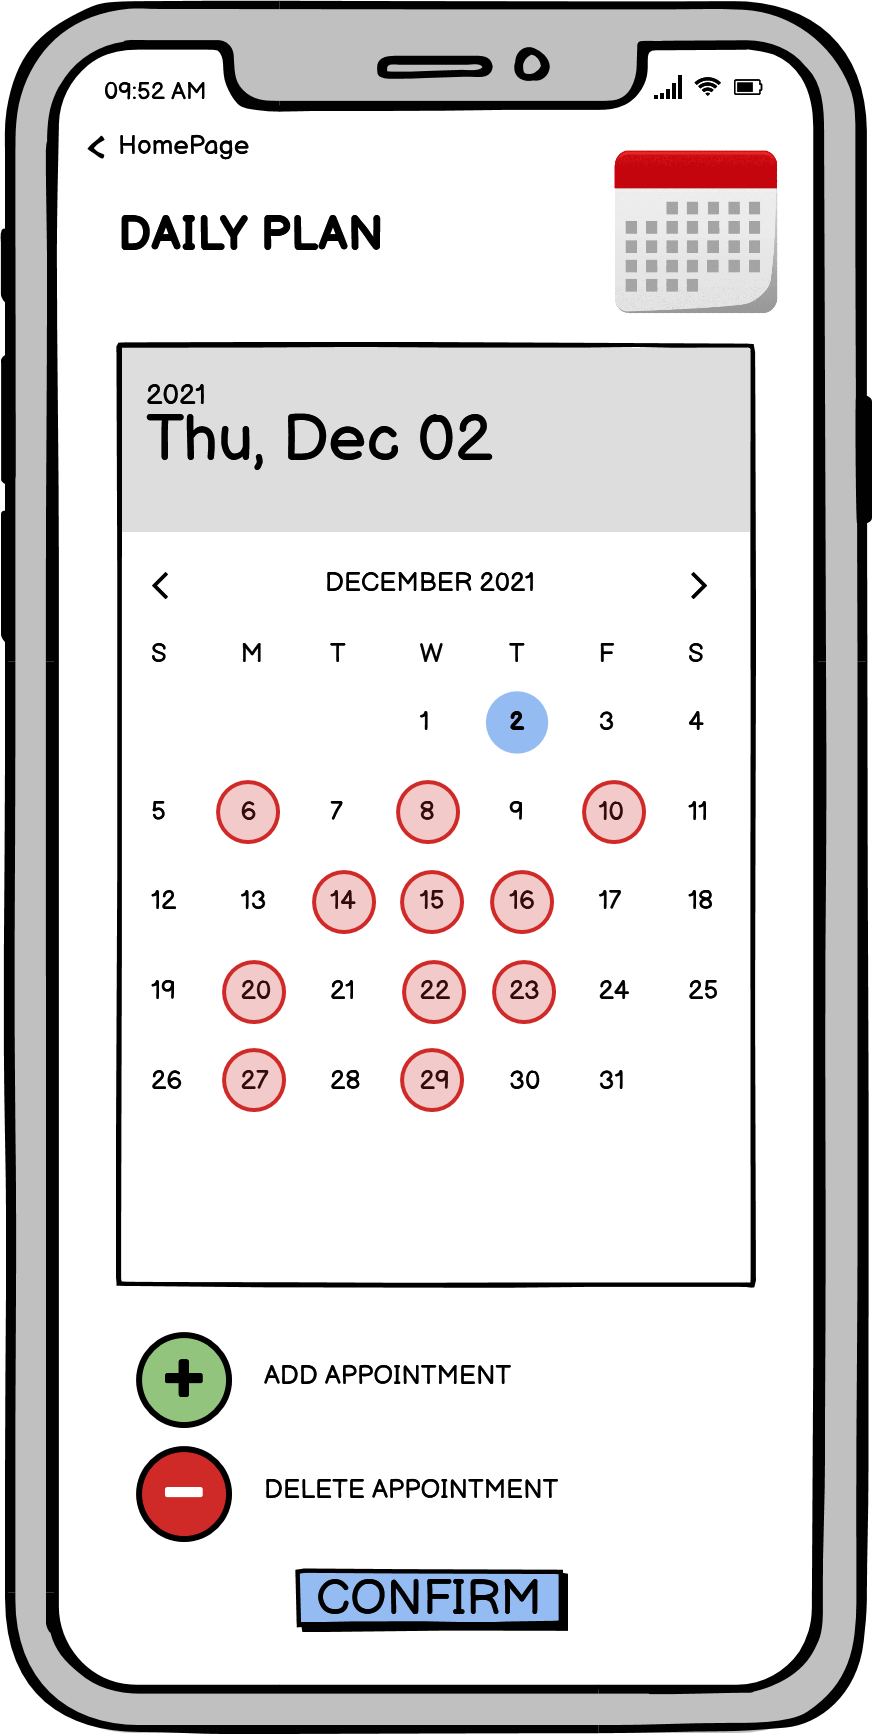
\includegraphics[scale=0.40]{Images/dailyplan.png}
    \caption{Daily plan management home page}
\end{figure}


\bigskip
\subsection{Functional Requirements}
\subsubsection{Goal-Requirement mapping}
\begin{description}
    \item [G1] The app should help and improve farmers' work-related activity
        \begin{description}
            \item[R1] The system shall keep track of the farmer who requested help and of the suggestion that they received
            \item[R2] The system shall keep track of historical data for each zone
            \item[R3] The system shall keep track of meteorological events
            \item[R4] Farmers shall be able to create a help request for the agronomist specifying the type of problem
            \item[R5] The system shall be able to record data about production inserted by the farmer
            \item[R7] Farmers shall be able to create discussion threads on the forum
            \item[R8] Farmers shall be able to reply to discussion on the forum
            \item[R9] The system shall send a notification to the Agronomists when a farmer has requested help
            \item[R10] After an agronomist has registered a best practice or a suggestion to a farmer, the system should infer the farmers with similar characteristics and send them the same suggestion
            \item[R11] The systems shall be able to connect to an external service to retrieve meteorological forecasts
            \item[R12] The system shall give Farmers the possibility to see weather forecasts
            \item[R13] The system shall be able to manage a forum
            \item[R14] The system shall be able to record data about visits of agronomists
            \item[R17] The system shall give Farmers the possibility to register
            \item[R18] The system shall give Farmers the possibility to login
            \item[R19] The system shall give the Farmers the possibilty to visualize personalized suggestion
            \item[R20] Agronomists shall be able to reply to discussion on the forum
            \item[R27] Agronomists shall be able to insert best practices discovered during inspections
            \item[R31] The system shall be able to localize and keep track of each farm 
 
 
        \end{description}
    \item [G2] The app should allow agronomists to oversee and improve farmers work
        \begin{description}
            \item[R1] The system shall keep track of the farmer who requested help and of the suggestion that they received
            \item[R2] The system shall keep track of historical data for each zone
            \item[R3] The system shall keep track of meteorological events
            \item[R4] Farmers shall be able to create a help request for the agronomist specifying the type of problem 
            \item[R5] The system shall be able to record data about production inserted by the farmer
            \item[R6] Agronomist shall be able to insert significant prodution thresholds for each zone
            \item[R7] Farmers shall be able to create discussion threads on the forum 
            \item[R9] The system shall send a notification to the Agronomists when a farmer has requested help
            \item[R10] After an agronomist has registered a best practice or a suggestion to a farmer, the system should infer the farmers with similar characteristics and send them the same suggestion
            \item[R11] The systems shall be able to connect to an external service to retrieve meteorological forecasts
            \item[R13] The system shall be able to manage a forum
            \item[R14] The system shall be able to record data about visits of agronomists
            \item[R15] The system shall be able to manage a calendar
            \item[R16] The system shall organize Agronomists' calendar in such a way that they visit each farm at least twice a year
            \item[R19] The system shall give the Farmers the possibilty to visualize personalized suggestion
            \item[R20] Agronomists shall be able to reply to discussion on the forum
            \item[R21] The system shall give Agronomists the possibility to see weather forecasts
            \item[R22] Agronomists shall be able to add or remove an appointment from daily plan
            \item[R23] At the end of each day Agronomists shall be able to confirm or communicate deviations from the daily plan
            \item[R24] The system shall give Agronomists the possibility to register
            \item[R25] The system shall give Agronomists the possibility to login
            \item[R26] Agronomists shall be able to visualize farmers' performance through the dashboard
            \item[R27] Agronomists shall be able to insert best practices discovered during inspections
            \item[R28] Agronomists shall be able to visualize disussion on the forum
            \item[R29] The system shall be able to keep track of all the areas and the agronomist responsible for them
            \item[R30] The system shall give Agronomists the possibility to know every farmer for which he is responsible 

 
 
        \end{description}
    \item [G3] The app should allow policymakers to control agriculture performance in Telangana
        \begin{description}
            \item[R1] The system shall keep track of the farmer who requested help and of the suggestion that they received
            \item[R2] The system shall keep track of historical data for each zone
            \item[R3] The system shall keep track of meteorological events
            \item[R5] The system shall be able to record data about production inserted by the farmer
            \item[R6] Agronomist shall be able to insert significant prodution thresholds for each zone   
            \item[R14] The system shall be able to record data about visits of agronomists
            \item[R31] The system shall be able to localize and keep track of each farm  
            \item[R32] The system shall give Policymakers the possibility to register 
            \item[R33] The system shall give Policymakers the possibility to login
            \item[R34] Policymaker shall be able to visualize farmers' performance through the dashboard
            \item[R35] Policymaker shall be able to visulize data inserted by farmers and agronomists
            \item[R36] Policymaker shall be able to visualize comparative performance of the farmers who received help
            \item[R37] The system shall give policymakers the ability to identify well-performing and underperforming farmers    
        \end{description}
\end{description}


\bigskip
\subsubsection{Scenarios}
\paragraph{Scenario 1} Daily plan confirmation\\
Tom is an agronomist that has just finished his work shift, so he logs in to the app and clicks on the daily plan icon.
The daily appointment with farmers just completed, follows exactly the plan previously determined, so he presses the
confirmation button.

\paragraph{Scenario 2} Daily plan modification\\
Martha is an agronomist that is planning his appointments with farmers. She logs in to DREAM and, from the home page,
opens the daily plan section; here she decided to remove an appointment planned for the 10th of December selecting the
corresponding date and then the deletion icon that updates the daily plan. After that, Martha, from the calendar,
selects the 28th of December, and then she presses on the addition icon below: doing that another section is opened in
which she can insert information about the appointment to plan (date, time, and the farm that she wants to visit).
Confirming the operation, she will come back to the daily plan section and the daily plan is updated.

\paragraph{Scenario 3} Agronomist's area selection\\
Marvin is an agronomist that has just completed the registration. After the registration and the log in,
he decides to select his area of responsibility from the map icon on the home page. In this area, a political map of
Telangana is shown and Marvin selects his responsibility zone. No errors occur so Marvin can select the confirmation
button and his area is stored.

\paragraph{Scenario 4} Forum discussion creation\\
Anthony is a farmer and has problems with soil humidity in his fields, so he decides to post a question on the forum.
In order to do that, he logs in and clicks on the forum icon. In the forum section, he selects the add discussion icon:
another section is opened in which he writes his question and post it.

\paragraph{Scenario 5} Farmer insert data\\
Jack is a farmer who recently finished collecting his harvest. He opens the app, logs in to the system. On his home page, 
he selects the Insert Data icon, he now can insert the amount and the type of crop he has harvested and then confirm.


\paragraph{Scenario 6} Farmer Help Request\\
Marty is a farmer who is having some problems in the cultivation of a crop and because he can't wait for a response on the 
forum decides to request help from an agronomist. He logs in on the app, selects the request help icon, inserts a brief description 
of the problem and then confirms that he wants to ask for the help of an agronomist. Victor is one of the agronomists responsible 
for the zone of Marty. After Marty's request, he receives a message containing a description of the problem. Victor conveys that the 
problem of Marty is a serious one so he decides to schedule a visit to his farm through the app functionality.

\paragraph{Scenario 7} Policymaker checks performance of farmer who received help\\
Tom is an official of the Telangana Department of Agriculture, after the recent flood he wants to know how many farmers have requested 
help and if this help has been effective. He logs in on the website of DREAM and can see the dashboard with some aggregate data. 
To see which farmers requested help he can select the previous month from the choice box and check which user had requested help, 
then he can see if in the current month the users who received help have overcome the thresholds set by the agronomist. He then wants 
to know who are the best performing farmers so he orders the table to show the users who have the greatest number of meteorological 
events but overcome the threshold nevertheless.

\newpage

\subsubsection{Use cases}

\begin{table}[H]
    \begin{tabu} to \textwidth {|X|X[4]|}
        \hline
        Name            & User creates an account \\ \hline
        Actor           & User                    \\ \hline
        Entry condition & \begin{itemize}
            \item The User has not created an account yet
            \item The User has to be a farmer, an agronomist or a policy maker
        \end{itemize}  \\ \hline
        Event flow      & \begin{enumerate}
            \item The User opens the app
            \item The app asks for login or registration
            \item The User clicks on \emph{"Register now"}
            \item The User inserts his first name, last name, username, e-mail, password and role
            \item The User clicks on \emph{"Register"}
            \item The app notifies to User that the registration is confirmed
        \end{enumerate}  \\ \hline
        Exit condition  & \begin{itemize}
            \item User account is added to the database
            \item The User can login
        \end{itemize}  \\ \hline
        Exceptions      & \begin{itemize}
            \item The User already exists
        \end{itemize}  \\ \hline
    \end{tabu}
\end{table}
\newpage

\begin{table}[H]
    \begin{tabu} to \textwidth {|X|X[4]|}
        \hline
        Name            & User logs in           \\ \hline
        Actor           & Registered User        \\ \hline
        Entry condition & \begin{itemize}
            \item The User has an account
        \end{itemize} \\ \hline
        Event flow      & \begin{enumerate}
            \item The User opens the app
            \item The app asks for login or registration
            \item The User inserts their username and password
            \item The User clicks on \emph{"Log-In"}
            \item The User receives confirmation from the server
            \item The Customer is brought to the home page
        \end{enumerate} \\ \hline
        Exit condition  & \begin{itemize}
            \item The User is logged in
            \item The User can use other features
        \end{itemize} \\ \hline
        Exceptions      & \begin{itemize}
            \item The User insert wrong credentials
            \item The insert username doesn't exist in the app database
        \end{itemize} \\ \hline
    \end{tabu}
\end{table}

\begin{table}[H]
    \begin{tabu} to \textwidth {|X|X[4]|}
        \hline
        Name            & User checks weather forecasts and suggestions           \\ \hline
        Actor           & Agronomist and farmer logged-in    \\ \hline
        Entry condition & \begin{itemize}
            \item The User has logged in
        \end{itemize} \\ \hline
        Event flow      & \begin{enumerate}
            \item The User presses on \emph{"Weather forecasts"} icon
            \item The User is brought to the \emph{"Weather forecasts"} page
            \item The User inserts the interested area and day
            \item The User visualizes the weather forecasts
            \item The User visualizes personalized suggestions
            \item The User return to the homepage
        \end{enumerate} \\ \hline
        Exit condition  & \begin{itemize}
            \item The User can use other features
        \end{itemize} \\ \hline
        Exceptions      & \begin{itemize}
            \item The inserted area doesn't exist
        \end{itemize} \\ \hline
    \end{tabu}
\end{table}

\begin{table}[H]
    \begin{tabu} to \textwidth {|X|X[4]|}
        \hline
        Name            & User answers forum discussions           \\ \hline
        Actor           & Agronomist and farmer logged-in    \\ \hline
        Entry condition & \begin{itemize}
            \item The User has logged in
        \end{itemize} \\ \hline
        Event flow      & \begin{enumerate}
            \item The User presses on \emph{"Forum"} icon
            \item The User is brought to the \emph{"Forum"} page
            \item The User scrolls the page and presses on an open discussion
            \item The User answers using his knowledge
            \item The app creates an answer with the creator username, the date and the time
            \item The user can choose to answer another discussion or return to the homepage
        \end{enumerate} \\ \hline
        Exit condition  & \begin{itemize}
            \item The User can use other features
        \end{itemize} \\ \hline
        Exceptions      & \begin{itemize}
            \item The answer is empty
        \end{itemize} \\ \hline
    \end{tabu}
\end{table}

\begin{table}[H]
    \begin{tabu} to \textwidth {|X|X[4]|}
        \hline
        Name            & Farmer asks for help          \\ \hline
        Actor           & Farmer logged-in   \\ \hline
        Entry condition & \begin{itemize}
            \item The Farmer has logged in
        \end{itemize} \\ \hline
        Event flow      & \begin{enumerate}
            \item The Farmer presses on \emph{"Help request"} icon
            \item The Farmer is brought to the \emph{"Help request"} page
            \item The Farmer inserts a brief description of the problem
            \item The Farmer specify the area in which his farm is located
            \item The Farmer clicks on \emph{"Send request"}
            \item The app forwards the request to the agronomist responsible for that area
            \item The app notify to the Farmer that the request has been sent
            \item The Farmer is brought to the homepage
        \end{enumerate} \\ \hline
        Exit condition  & \begin{itemize}
            \item The Farmer can use other features
        \end{itemize} \\ \hline
        Exceptions      & \begin{itemize}
            \item The request is empty
            \item There is no agronomist responsible for that area
        \end{itemize} \\ \hline
    \end{tabu}
\end{table}

\begin{table}[H]
    \begin{tabu} to \textwidth {|X|X[4]|}
        \hline
        Name            & Agronomist selects the area he is responsible for          \\ \hline
        Actor           & Agronomist logged-in   \\ \hline
        Entry condition & \begin{itemize}
            \item The Agronomist has logged in
        \end{itemize} \\ \hline
        Event flow      & \begin{enumerate}
            \item The Agronomist press on \emph{"Select your area"} icon
            \item The Agronomist is brought to the \emph{"Select your area"} page
            \item The app opens a map of Telangana's State divided by areas 
            \item The Agronomist press on the area he is responsible for
            \item The app notify to the Agronomist that the operation was successful
            \item The Agronomist is brought to the homepage
        \end{enumerate} \\ \hline
        Exit condition  & \begin{itemize}
            \item The Agronomist can use other features
            \item The selected area is added to the database
        \end{itemize} \\ \hline
        Exceptions      & \begin{itemize}
            \item The selected area has already been taken
        \end{itemize} \\ \hline
    \end{tabu}
\end{table}

\begin{table}[H]
    \begin{tabu} to \textwidth {|X|X[4]|}
        \hline
        Name            & Users logs out        \\ \hline
        Actor           & Users logged-in   \\ \hline
        Entry condition & \begin{itemize}
            \item The User has logged in
        \end{itemize} \\ \hline
        Event flow      & \begin{enumerate}
            \item The User press on \emph{"Settings"} icon
            \item The User is brought to the \emph{"Settings"} page
            \item The User press on \emph{"Log-out"} button
            \item The User is brought to the \emph{"Log-in"} page
        \end{enumerate} \\ \hline
        Exit condition  & \begin{itemize}
            \item The User is logged out
        \end{itemize} \\ \hline
    \end{tabu}
\end{table}

\newpage

\begin{table}[H]
    \begin{tabu} to \textwidth {|X|X[4]|}
        \hline
        Name            & Agronomist adds appointment      \\ \hline
        Actor           & Agronomist                      \\ \hline
        Entry condition & \begin{itemize}
            \item The Agronomist is logged in
        \end{itemize} \\ \hline
        Event flow      & \begin{enumerate}
            \item The Agronomist opens the \emph{"Daily Plan"} section
            \item The Agronomist is brought to a page with a calendar 
            \item The Agronomist selects the day that we wants to modify
            \item The Agronomist presses the \emph{Add appointment} button
            \item The Agronomist inserts additional information about the visit
            \item The Agronomist presses the \emph{Confirm} button
            \item The Agronomist receives confirmation from the server
        \end{enumerate} \\ \hline
        Exit condition  & \begin{itemize}
            \item The new event is added to the calendar of the agronomist
            \item Agronomist can see the new event on the calendar
        \end{itemize} \\ \hline
        Exceptions      & \begin{itemize}
            \item The day is already full
        \end{itemize} \\ \hline
    \end{tabu}
\end{table}

\begin{table}[H]
    \begin{tabu} to \textwidth {|X|X[4]|}
        \hline
        Name            & Farmer creates forum discussion  \\ \hline
        Actor           & Farmer                      \\ \hline
        Entry condition & \begin{itemize}
            \item The Farmer is logged in
        \end{itemize} \\ \hline
        Event flow      & \begin{enumerate}
            \item The Farmer opens the \emph{"Forum"} section
            \item The Farmer is brought to the \emph{"Forum"} page 
            \item The Farmer presses the \emph{Create Discussion} button
            \item The Farmer inserts the question and additional information
            \item The Farmer presses the \emph{Confirm} button
            \item The Farmer receives confirmation from the server
        \end{enumerate} \\ \hline
        Exit condition  & \begin{itemize}
            \item The new discussion is added to the forum
            \item The Farmer can see his question on the forum
        \end{itemize} \\ \hline
        Exceptions      & \begin{itemize}
            \item The question is empty
        \end{itemize} \\ \hline
    \end{tabu}
\end{table}

\begin{table}[H]
    \begin{tabu} to \textwidth {|X|X[4]|}
        \hline
        Name            & Farmer inserts data  \\ \hline
        Actor           & Farmer                      \\ \hline
        Entry condition & \begin{itemize}
            \item The Farmer is logged in
        \end{itemize} \\ \hline
        Event flow      & \begin{enumerate}
            \item The Farmer opens the \emph{Insert Data} section
            \item The Farmer is brought to the \emph{Insert Data Form} 
            \item The Farmer compiles the form inserting the type of crop the amount of crop and the amount of water used
            \item The Farmer presses the \emph{Confirm} button
            \item The Farmer receives confirmation from the server
        \end{enumerate} \\ \hline
        Exit condition  & \begin{itemize}
            \item The new production data is added to the database
        \end{itemize} \\ \hline
        Exceptions      & \begin{itemize}
            \item The Farmer inserted invalid data
        \end{itemize} \\ \hline
    \end{tabu}
\end{table}

\begin{table}[H]
    \begin{tabu} to \textwidth {|X|X[4]|}
        \hline
        Name            & Agronomist inserts threshold  \\ \hline
        Actor           & Agronomist                     \\ \hline
        Entry condition & \begin{itemize}
            \item The Agronomist is logged in
        \end{itemize} \\ \hline
        Event flow      & \begin{enumerate}
            \item The Agronomist opens the \emph{Dashboard} section
            \item The Agronomist is brought to the \emph{Dashboard} page 
            \item The Agronomist presses on the \emph{insert threshold} button
            \item The Agronomist is brought to the \emph{Insert Threshold form}
            \item The Agonomist insert the threshold
            \item The Agronomist receives confirmation from the server
        \end{enumerate} \\ \hline
        Exit condition  & \begin{itemize}
            \item The new threshold is added to the database
        \end{itemize} \\ \hline
        Exceptions      & \begin{itemize}
            \item The Agronomist inserted invalid data
        \end{itemize} \\ \hline
    \end{tabu}
\end{table}


\begin{table}[H]
    \begin{tabu} to \textwidth {|X|X[4]|}
        \hline
        Name            & Policymaker sees dashboard  \\ \hline
        Actor           & Policymaker                \\ \hline
        Entry condition & \begin{itemize}
            \item The Policymaker is logged in
        \end{itemize} \\ \hline
        Event flow      & \begin{enumerate}
            \item The Policymaker opens the \emph{Dashboard} section
            \item The Policymaker is brought to the \emph{Dashboard} page 
            \item The Policymaker presses on the \emph{water used column} of the table to order the farmer by water used 
            \item The Policymaker see the table and decides the farmer to reward
        \end{enumerate} \\ \hline
        Exceptions      & \begin{itemize}
            \item The Table is empty
        \end{itemize} \\ \hline
    \end{tabu}
\end{table}

\newpage

\begin{table}[H]
    \begin{tabu} to \textwidth {|X|X[4]|}
        \hline
        Name            & Agronomist replies to help request \\ \hline
        Actor           & Agronomist                     \\ \hline
        Entry condition & \begin{itemize}
            \item The Agronomist is logged in
        \end{itemize} \\ \hline
        Event flow      & \begin{enumerate}
            \item The Agronomist receives an help request
            \item The Agronomist open the \emph{Help Request} section
            \item The Agronomist sees a list of help requests
            \item The Agronomist select the help request he want to answer
            \item The Agronomist insert an answer to the problem
            \item The Agronomist presses \emph{Send} button
            \item The Agronomist receives confirmation from the server
        \end{enumerate} \\ \hline
        Exit condition  & \begin{itemize}
            \item The answer is sent to the farmer
            \item The Agronomist can visualize his answer
        \end{itemize} \\ \hline
        Exceptions      & \begin{itemize}
            \item The Agronomist answer is empty
        \end{itemize} \\ \hline
    \end{tabu}
\end{table}

\newpage
\subsection{Sequence diagrams}
\begin{figure}[H]
    \centering
    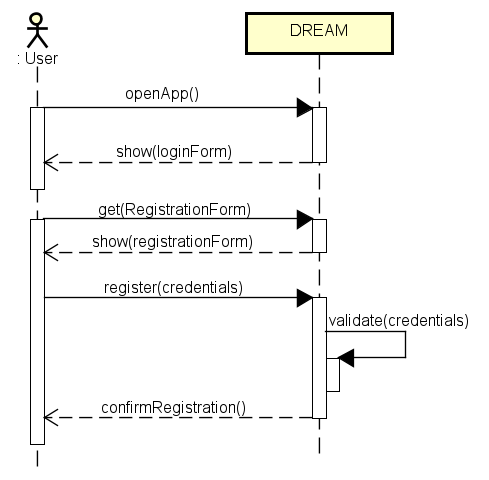
\includegraphics[scale=0.7]{Images/RegistrationSequence.png}
    \caption{Registration sequence diagram}
\end{figure}

\bigskip
\begin{figure}[H]
    \centering
    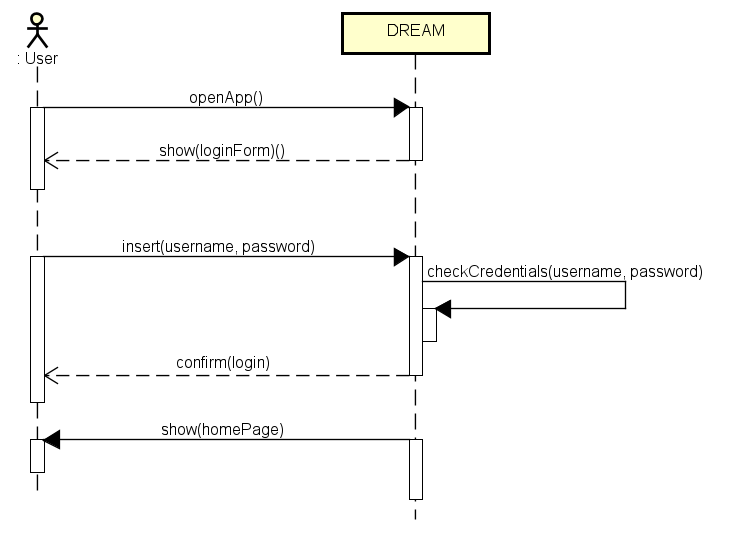
\includegraphics[scale=0.7]{Images/login.png}
    \caption{Log-in sequence diagram}
\end{figure}

\bigskip
\begin{figure}[H]
    \centering
    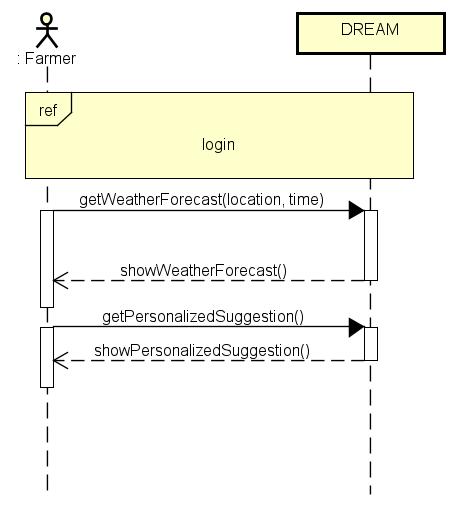
\includegraphics[scale=0.7]{Images/ChecksWeatherForecastSequence.png}
    \caption{Sequence diagram of weather forecast check}
\end{figure}

\bigskip
\begin{figure}[H]
    \centering
    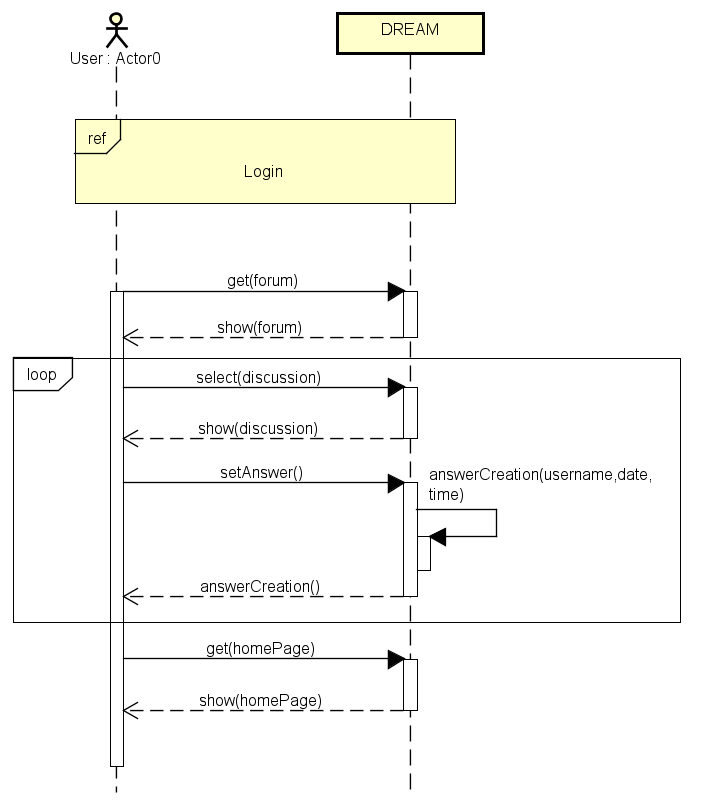
\includegraphics[scale=0.7]{Images/userAnswersForumDiscussion.png}
    \caption{Sequence diagram of users' answer on the forum}
\end{figure}

\bigskip
\begin{figure}[H]
    \centering
    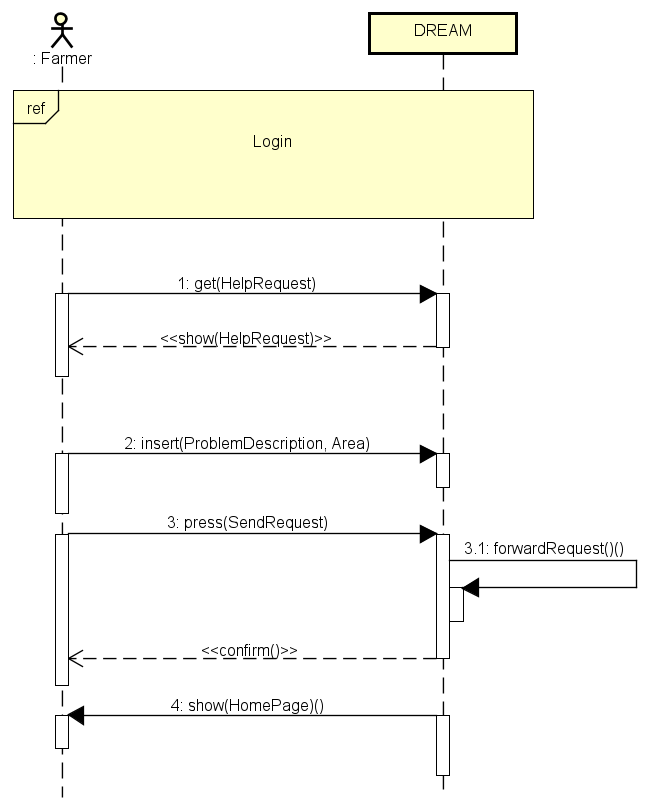
\includegraphics[scale=0.7]{Images/helpRequest.png}
    \caption{Farmer requesting help sequence diagram}
\end{figure}

\bigskip
\begin{figure}[H]
    \centering
    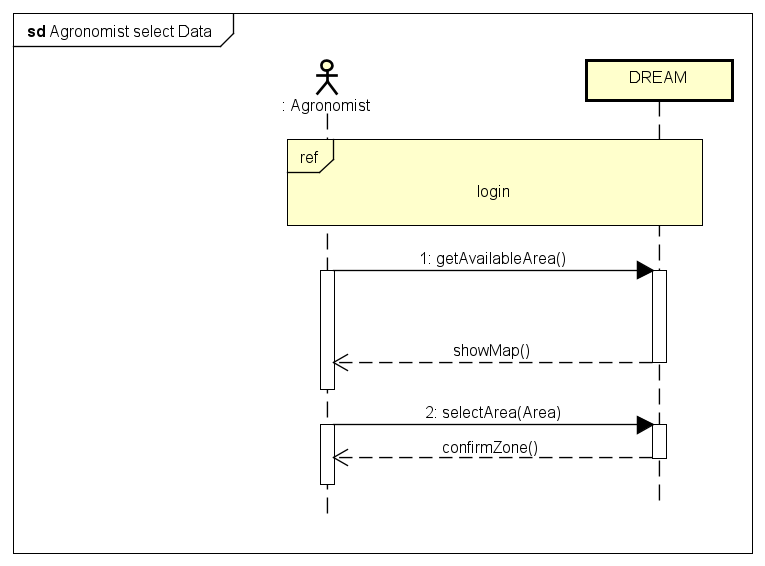
\includegraphics[scale=0.7]{Images/AgronomistSelectDataSequence.png}
    \caption{Sequence diagram of the area selection}
\end{figure}

\bigskip
\begin{figure}[H]
    \centering
    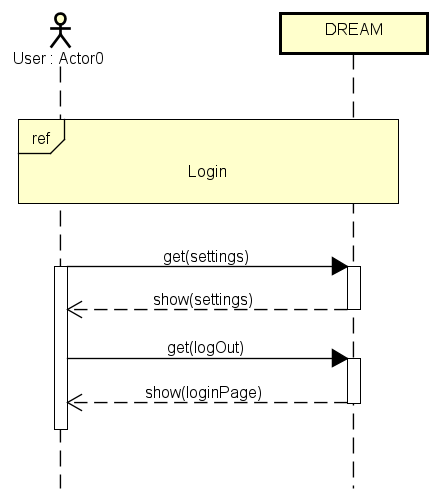
\includegraphics[scale=0.7]{Images/userLogsOut.png}
    \caption{Sequence diagram of log out}
\end{figure}

\bigskip
\begin{figure}[H]
    \centering
    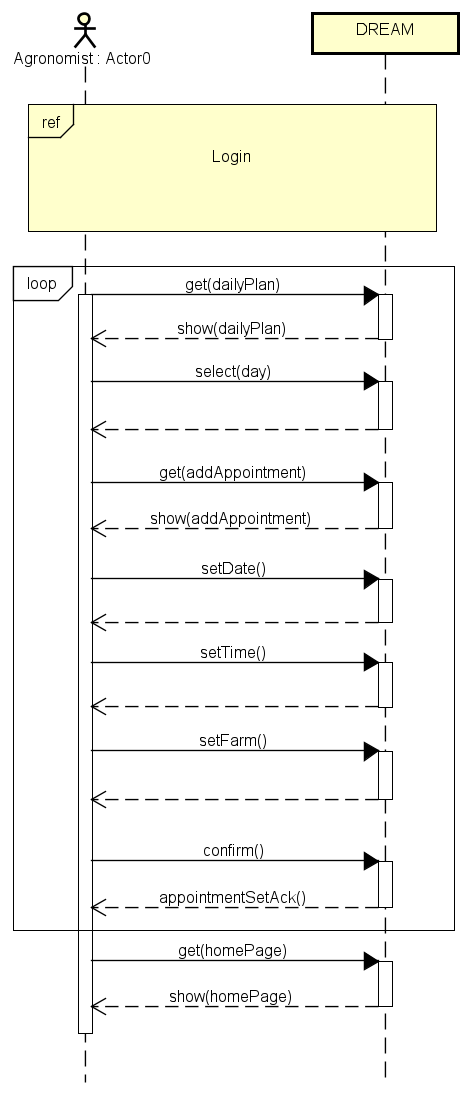
\includegraphics[scale=0.6]{Images/agronomistAddsAppointment.png}
    \caption{Sequence diagram of the addition of an appointment}
\end{figure}

\bigskip
\begin{figure}[H]
    \centering
    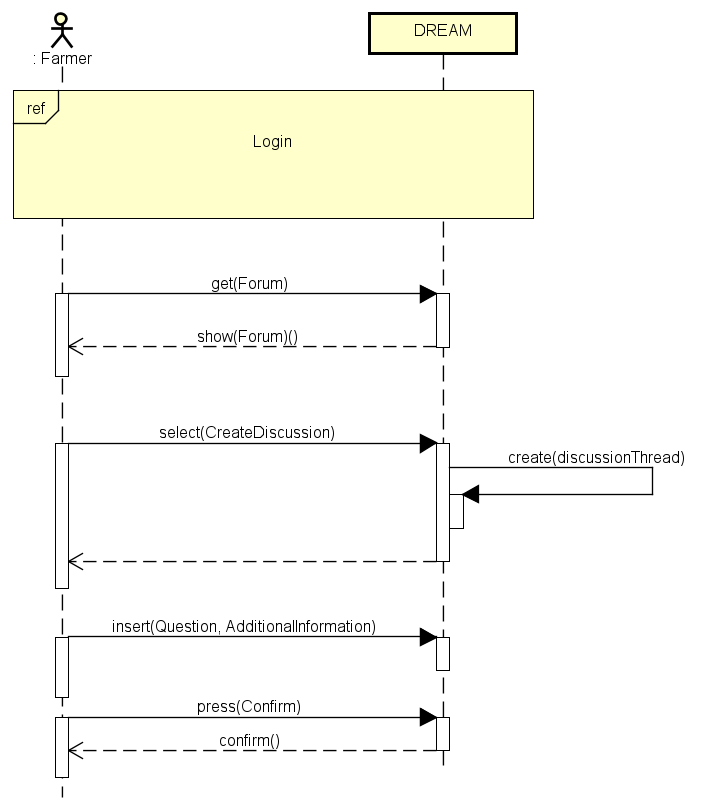
\includegraphics[scale=0.7]{Images/createDiscussion.png}
    \caption{Sequence diagram of the creation of a discussion on the forum}
\end{figure}

\bigskip
\begin{figure}[H]
    \centering
    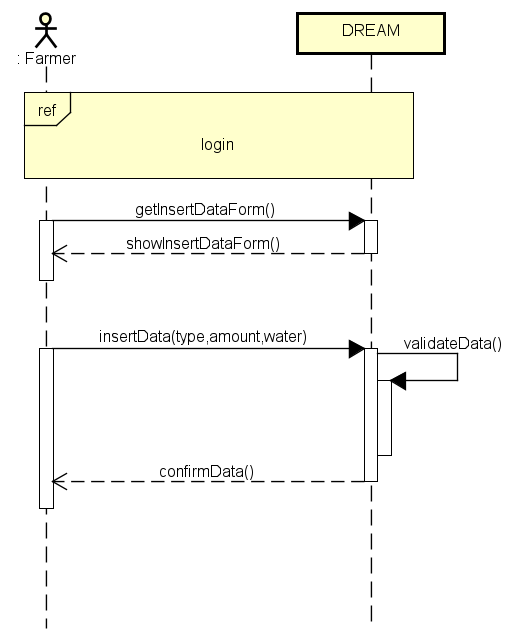
\includegraphics[scale=0.7]{Images/FarmerInsertsDataSequence.png}
    \caption{Farmer insert data concerning production, sequence diagram}
\end{figure}

\bigskip
\begin{figure}[H]
    \centering
    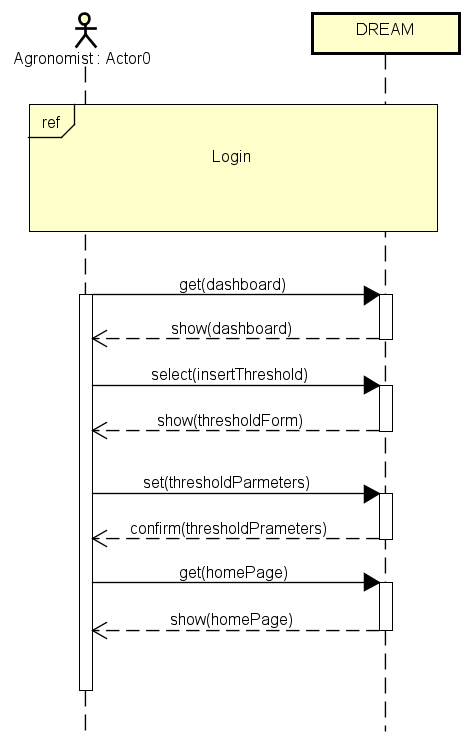
\includegraphics[scale=0.7]{Images/agronomistCreatesThreshold.png}
    \caption{Sequence diagram of threshold creation by an agronomist}
\end{figure}

\bigskip
\begin{figure}[H]
    \centering
    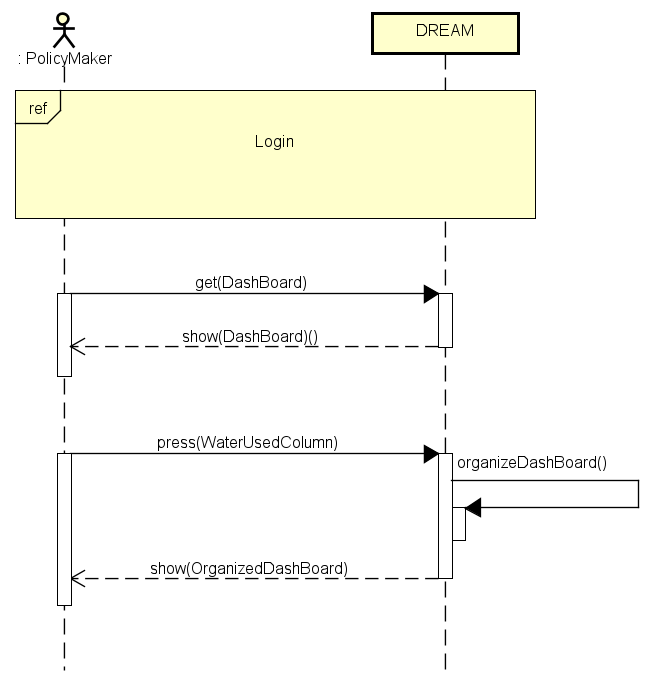
\includegraphics[scale=0.7]{Images/seeDashBoard.png}
    \caption{Sequence diagram of dashboard check by policy maker}
\end{figure}

\bigskip
\begin{figure}[H]
    \centering
    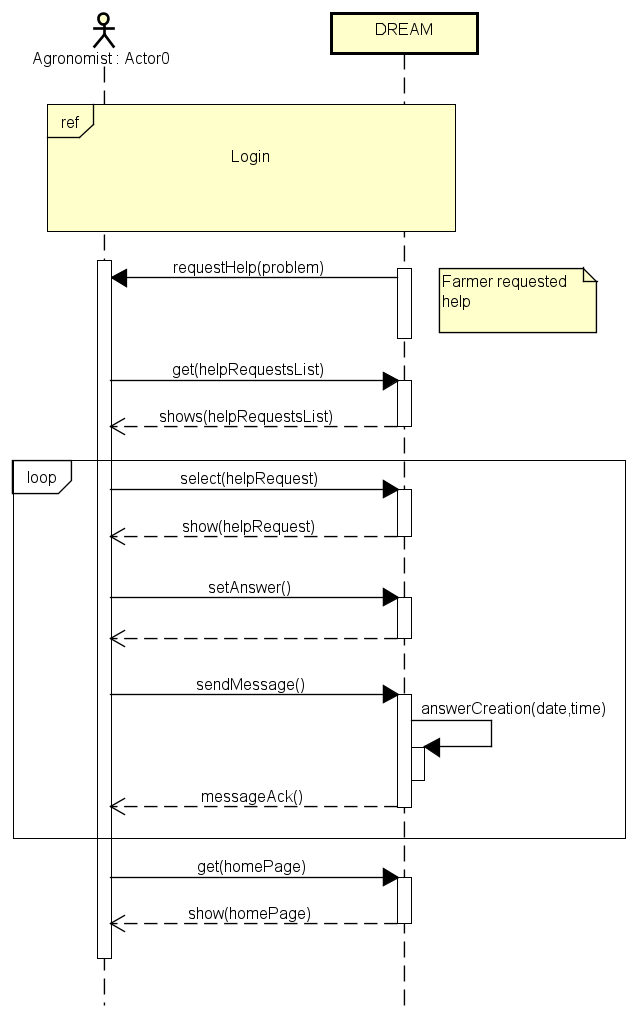
\includegraphics[scale=0.7]{Images/agronomistAnswersHelpRequests.png}
    \caption{Sequence diagram of an agronomist replying to help requests}
\end{figure}

\newpage
\subsection{Performance Requirements}
Though in these cases time is not critical, the requested performances are:
\begin{itemize}
    \item Weather forecasts update must be done within 5 seconds.
    \item When farmer adds production data on the app, the server should be updated within 15 seconds.
    \item When someone answers or requests help on the forum, its post need to be add within 10 seconds.
    \item Daily plan modifications have to be scheduled within 0.5 seconds.
    \item Private help requests and answers, need to be sent to the receiver within 3 seconds.
\end{itemize}


\subsection{Design constraints}
\subsubsection{Hardware limitations}
Running \emph{DREAM} requires a smartphone or computer and a web connection.

\subsection{Software System Attributes}
\subsubsection{Reliability}
\emph{DREAM} should be available 24/7, except for maintenance that has to be performed
only at night and has to last no longer than 2 hours.
\newline The highest number of simultaneous accesses is expected in the harvest time.

\subsubsection{Availability}
The system must be available as much as possible; hence, during daytime is required a minimum value of 97\%.
During the night the availability could be lowered to 95\%.

\subsubsection{Security}
The most critical problems concerning security are privacy, data integrity and authentication. For instance a
MITM attack between policymaker and the server could be dangerous for private data. In order to overcome all
these security problems, the communication between parties should be encrypted through HTTPS protocol.

\subsubsection{Maintainability}
The system must be designed in such a way that permits future addition of functionalities with minimum effort.

\subsubsection{Portability}
\emph{DREAM} should be easily deployable on a dedicated machine, on a virtual private server or on a cloud.
It is in any case usable on every web browser, from every device. The mobile application must be supported by iOS
and Android.